\documentclass{beamer}
\usepackage[orientation=portrait,size=a0,scale=1.4,debug]{beamerposter}
\mode<presentation>{\usetheme{ZH}}
\usepackage[utf8]{inputenc}
\usepackage[spanish, english]{babel} 
\usepackage{siunitx} 
\usepackage{hyperref} 
\usepackage{wrapfig}
\usepackage{graphicx}
\usepackage{enumerate}
\usepackage{ragged2e}
\usepackage[font=scriptsize,justification=justified]{caption}
\usepackage{array,booktabs,tabularx}
\newcolumntype{Z}{>{\centering\arraybackslash}X} 
\sisetup{per=frac,fraction=sfrac}
\title{\huge Inducción de corriente eléctrica en bobinas de Helmholtz}
\author{Gamaliel López Padilla}
\institute[FCFM]{Facultad de Ciencias Fisico Matematicas}
\date{19 abril 2018}
\newlength{\columnheight}
\setlength{\columnheight}{104cm}
\begin{document}
\begin{columns}
\begin{column}{.50\textwidth}
\begin{beamercolorbox}[center]{postercolumn}
\begin{minipage}{.98\textwidth}  
\parbox[t][\columnheight]{\textwidth}{ 
\vspace*{1cm}
\begin{myblock}{Abstract}
Se comprobara experimentalmente la relación lineal entre la corriente eléctrica inducida por una fuerza electromotriz generada por un generador de ondas y el potencial eléctrico inducido por un campo magnético producido por una bobina de Helmholtz, en donde las dos bobinas estaran separadas una distancia equivalente a su radio y sus centros estaran sobre un mismo eje, las dos bobinas tendran el mismo espesor y el mismo número de vueltas de alambre en ellas.
\end{myblock}
\begin{myblock}{Introducción}
Las bobinas de Helmholtz son una estructura constituida por dos carretes o bobinas conformadas por un gran número de espiras exactamente iguales separadas entre sí; cuyo fin es obtener un campo magnético unifrme en un volumen determinado por el espacio ubicado entre el punto medio del segmento que une a los centros de las bobinas y las regiones cercanas a las mismas cuando existe una intensidad de corriente.\\
Michael Faraday y Joseph Henry realizaron experimentos en donde un conductor que se mueve puede varias las lineas de fuerza de un campo magnético, lo cual origina una fuerza electromotriz (fem) inducida y en un circuito cerrado se originaria una corriente inducida, este mismo fenomeno sucede si un flujo magnético que atraviesa a un conductor es variable.
\end{myblock}
\begin{myblock}{Objetivo}
Comprobar experimentalmente la relación lineal entre la corriente eléctrica generada por una fuerza electromotriz y el potencial electrico producido por un campo magnético
\end{myblock}
\begin{myblock}{Marco Teórico}
El campo magnético debido a un solenoide con N espiras de radio R cuyo eje central esta colocado sobre el eje z, de modo que el centro de la bobina esta en (0,0,z).
\begin{equation}
B_z= \frac{N \mu_0 I}{2} \frac{R^2}{(R^2+z^2)^{3/2}}
\end{equation}
Calculando el campo magnético de un solenoide de longitud L, con N vueltas en el que pasa una 
corriente I. Se tomara dz' a una distancia z', sobre el eje z, por ese diferencial pasa una corriente 
\begin{equation*}
dI=N I dz'
\end{equation*}
Escribiendo la ecuación (1) en forma diferencial
\begin{equation}
dB_z = \frac{\mu_0 N I dz'}{2L} \frac{R^2}{(R^2+(z-z')^2)^{3/2}}
\end{equation}
Realizando la integral de $-a/2$ a $a/2$, donde a es el grosor de la bobina, se obtiene que:
\begin{equation}
B_z = \frac{\mu_0 N I}{2} \left \{ \frac{z+a/2}{\sqrt{R^2+(z+a/2)^2}} - \frac{z-a/2}{\sqrt{R^2+(z-a/2)^2}}\right \}
\end{equation}
Con este campo magnético provocado por la bobina numero 1, se podra obtener el flujo magnético que atraviesa a la bobina número dos. 
La definición de flujo magnético es:
\begin{equation}
\Phi_m = \int \vec{B} \cdot d\vec{S}
\end{equation}
Para obtener el flujo magnético sobre toda la superficie que se encuentra entre la bobina 1 hasta la bonina numero dos se integrara desde d a d+b, donde d es la distancia entre las bobinas y b es el grosor de la bobina número 2 y el $dS$ será cambiado por la el diferencial $2\pi r_2 dz'$ con lo que el flujo magnético es:\\
\changefontsizes{16pt}
\begin{center}
$\Phi_m = \mu_0 \pi  I_{max}( \sqrt{R^2+(R+3a/2)^2}-2\sqrt{R^2+(R+a/2)^2}+\sqrt{R^2+(R^2-a/2)^2})$
\end{center}
\normalize
El generador de ondas produce una corriente alterna, la cual depende del tiempo de la siguiente forma:
\begin{equation}
I(t)= I_{max} sin(\omega t)
\end{equation}
\end{myblock}
}\end{minipage}
\end{beamercolorbox}
\end{column}
\begin{column}{.50\textwidth}
\begin{beamercolorbox}[center]{postercolumn}
\begin{minipage}{.98\textwidth} 
\parbox[t][\columnheight]{\textwidth}{
\vspace*{1cm}
\begin{myblock}{Marco teórico}
La ley de Faraday-Henry describe el fenomeno conocido como "inducción electromagnética. Esta ley relaciona la fuerza electromotriz con la variación de flujo magnético en una espira, bobina o circuito de la siguiente manera:
\begin{equation}
 \epsilon= -\frac{d\Phi_B}{dt}
\end{equation}
La fem inducida en la bobina sera llamada $V_2$, con lo cual sera aplicada la ley de Faraday.
\begin{equation}
V_2 (t) = -  \omega \Phi_m cos(\omega t)
\end{equation}
\end{myblock}
\begin{myblock}{Método experimental}
Los materiales utilizados por los integrantes del equipo fueron:\\
$\cdot$ 2 Bobinas de Helmholtz\\
$\cdot$ Generador de ondas\\
$\cdot$ Cables para corriente\\
$\cdot$ Cinta métrica\\
$\cdot$ Multímetro\\
Las bobinas fueron ubicadas con una distancia igual a la los radios de las bobinas y que el centro de cada una coincidiera, la bobina número 1 fue conectada al generador de ondas, la cual le proporcionara una fuerza electromotriz, en la bobina numero 1 fue conectado un multímetro en serie para medir cual era la corriente eléctrica inducida, en cambio en la bobina número dos fue conectado un multímetro el cual media el potencial eléctrico.\\
Con los datos obtenidos se realizo la siguiente grafica:\\
\begin{center}
\begin{figure}
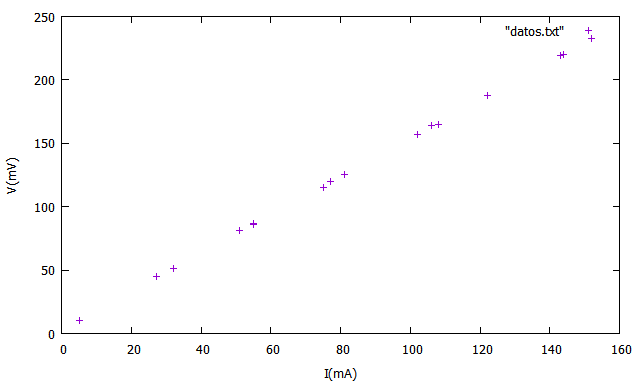
\includegraphics[scale=0.8]{images/grafica.png}
\caption{Datos obtenidos por los multímetros}
\end{figure}
\end{center}
Al aplicar el método de minimos cuadrados podemos entrar la relación existente entre la corriente eléctrica y el potencial eléctrico existente en la bobina número 2, la cual es:
\begin{equation*}
m=\frac{N \sum xy - \sum x \sum y}{N\sum x^2 -\sum x \sum x} = \frac{(19)(263989.25)-(2469.89)(1597)}{(19)(406090)-(2469.89)^2} = 0.66
\end{equation*}
Con lo que al comparar la recta $y=0.66x$ 
\begin{center}
\begin{figure}
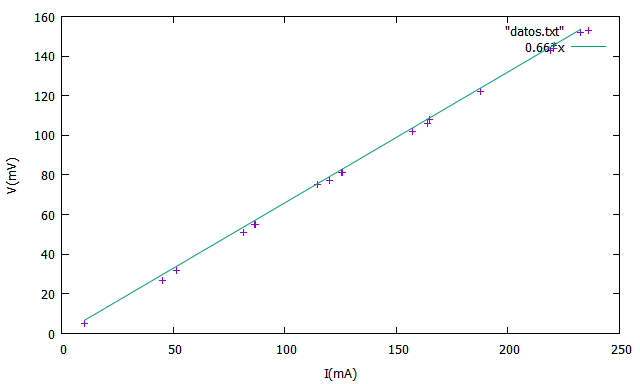
\includegraphics[scale=0.8]{images/grafica2.png}
\caption{Comparacion recta y=0.66x con los datos obtenidos}
\end{figure}
\end{center}
Calculando el coeficiente de correlación lineal de los datos se obtiene el valor:
\begin{equation*}
r_{xy}= \frac{N\sum xy - \sum x \sum y}{\sqrt{N\sum x^2 - (\sum x)^2 }*\sqrt{N\sum y^2 -(\sum{y})^2}}=...=0.99
\end{equation*}
\end{myblock}
\begin{myblock}{Resultados}
Como el coeficiente de correlación es muy cercano a 1, se comprueba que el potencial eléctrico en la bobina número dos es proporcional a la corriente eléctrica de la bobina número 1, y esa proporción es de 0.66, ese en nuestro sistema de bobinas.
\end{myblock}
\begin{myblock}{Referencias}
\small
$[1]$ Villalba, J., Ferrreira, L., Arribas, E., \& Beléndez Augusto. (2015, marzo 31).Estudio experimental de la inducción 	electromagnética entre dos bobinas: Dependencia con la corriente eléctrica, 37, 7. 10 abril 2018, De Revista 			Brasileira de Ensino de Física\\
$[2]$ Barbero,A. J.;J. A.; Mafé, S., "Induced EMF in a solenoid a simple quantitative verification of Faraday´s law". Physics Education 29 (1994) 102-105.\\
$[3]$ Manzanares, J. A.; Bisquert, J.; García Belmonte, G.; Fernández, M.; “An
experiment on voltage induction pulses”. American Journal of Physics 62
(1994) 702-706.
\end{myblock}
}
\end{minipage}
\end{beamercolorbox}
\end{column}
\end{columns}
\end{document}